\begin{figure}[h]
	\caption{An example of a bar chart}
	\centering
	\medskip

	\pgfplotsset{compat=newest}
	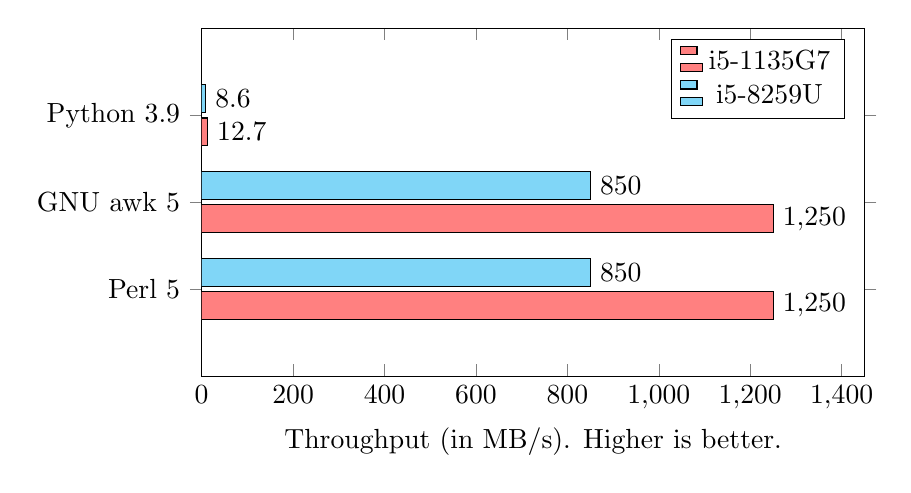
\begin{tikzpicture}
		\begin{axis}
			[ 
			xbar, 
			xmin=0, 
			width=10cm,
			height=6cm, 
			enlarge y limits=0.5, 
			xlabel={Throughput (in MB/s). Higher is better.},
			xmax=1450,
			%ylabel={Language},
			symbolic y coords={perl,gawk,python}, 
			yticklabels={Python 3.9,GNU awk 5,Perl 5},
			ytick=data,
			nodes near coords,
			nodes near coords align={horizontal}, 
			legend pos=north east
			]	
			\addplot[fill=red!50] coordinates {(12.7,python) (1250,gawk) (1250,perl)}; 
			\addplot[fill=cyan!50] coordinates {(8.6,python) (850,gawk) (850,perl)};
			\legend{i5-1135G7,i5-8259U};
		\end{axis} 
	\end{tikzpicture}
	\label{figure:throughput-comparison}
	
\end{figure}
